
% The titlepage
\pgfmathsetseed{1}
\newbox\mybox
{
\parindent0pt
\null
\thispagestyle{empty}
\vskip3cm
\vfill
\hfil

\begin{tikzpicture}[overlay,]

%Water mark
  %\node [rotate=60, scale=20, text opacity=0.2] at (current page.center) {Sample};
  %\draw [line width=3mm, opacity=.25] (current page.center) circle (6cm);

  \begin{pgfonlayer}{background}
    \coordinate (front) at (.06\paperwidth,.35\paperheight);
    \coordinate (bottom) at (0,-1\paperheight);
    \coordinate (sky) at (0,1\paperheight);
    \coordinate (left) at (-.51\paperwidth,0);
    \coordinate (right) at (1\paperwidth,0);
    \fill [bgorange] (bottom -| right) rectangle ([xshift=1mm, yshift=-1mm]front);
    \fill [rightgreen] ([xshift=1mm]front) rectangle (sky -| right);
    \fill [leftgreen] ([yshift=-1mm]front) rectangle (bottom -| left);
    \fill [leftgreen] (front) rectangle (sky -| left);
    \shade [left color=leftgreen,right color=rightgreen]
      ([xshift=1mm]front) rectangle (sky -| right);
  \end{pgfonlayer}

  \node [below right=1cm, scale=4, align=left] at (front) {\baselineskip=2pt $\mahtNotes\ of\ Mathematics$};
  \node [white, below=4.3cm, right=1.5cm, align=left, font=\sffamily] at (front) {\Huge \emph{Third Edition}};
  \node [above=1cm, right=1.5cm, align=left, font=\sffamily] at (front) {\Huge Hsin Anonym};

  \node [opacity=0.5] at (.55\paperwidth,-.15\paperheight) {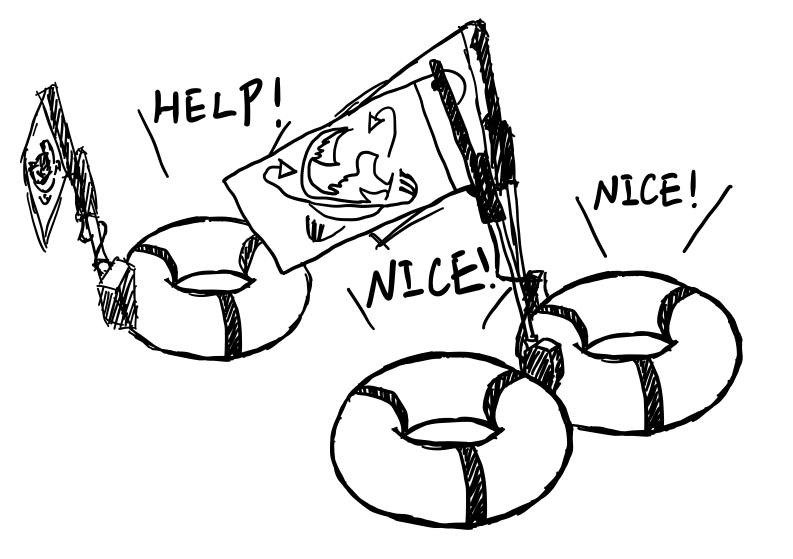
\includegraphics[scale=0.5]{Cover/Draftv.png}};
\end{tikzpicture}

\vfill
\vbox{}
\clearpage
}

\setlength{\headheight}{14pt}
\large
\setlength\parindent{2em}

\begin{titlepage}
   {\indent\fontsize{30pt}{0pt}\textbf{Notes of Mathematics}}

   \vfill
   {\indent\small{\textsc{Author: Hsin}}}\\
   {\indent\small{\textsc{E-Mail}: grammcyao@icloud.com}}\\
   {\indent\small{\textsc{Update}: \today}}
\end{titlepage}